\section{Background}
\label{sec:background}
This section generally introduces blockchain and consensus protocols, gives an overview of Algorand, and provides the pertinent Coq background.

\subsection{Blockchains and Consensus Protocols}

A blockchain is an ordered sequence of cryptographically linked blocks of records, in much the same way as links in a chain are firmly latched in sequence. A blockchain provides a persistent, tamper-proof and globally accessible ledger of transactions. It is built using well-established and publicly known cryptographic tools, including most importantly one-way hash functions [add pointer]. Anyone can verify the validity of its transactions, and no one can tamper with a transaction or claim a transaction that does not appear in the chain. 

This makes blockchains particularly well suited for building self-governing and autonomous distributed systems. Indeed, a blockchain is a key component for allowing a collection of nodes in a communication network (who do not necessarily trust each other) to work collectively and make decentralized decisions. Nevertheless, the nodes will need more than just a blockchain to achieve proper decentralized operation. Specifically, they need a mechanism for identifying and agreeing on the next block of transactions to be appended to the chain, a mechanism known as a consensus protocol.

A consensus protocol typically proceeds in rounds, where the objective of a round is to try to produce the next block and record it in the chain. As such, a consensus protocol includes both: 
(1) a mechanism for decentralized selection of one or more block proposers or producers of a round in the protocol, and 
(2) a mechanism for achieving decentralized consensus on a single block to be appended to the chain. 

In an idealistic (and rather unrealistic) setup, in which communication networks are perfectly reliable with zero-delay message delivery, and in which all participating nodes run error-free code and behave honestly, achieving consensus on a single block in each round is a trivial task. All nodes would instantaneously see all proposed blocks and their trusted opinions about them. In reality, however, the situation is actually very different. Distributed systems utilize global Internet (IP-based) communication networks, which are inherently unreliable and where significant message transmission delays are not uncommon. Furthermore, nodes may deviate from the protocol, either intentionally (when compromised by malicious users) or unintentionally (due to internal errors). These complications can hinder the consensus process, resulting potentially in the system being unusable or in losing large amounts of assets maintained by the system.

Therefore, consensus protocols need to maintain a consistent global view of the system while relying only on the local knowledge at the level of its individual (honest) nodes. Moreover, these protocols must ensure continuous and fair operation of the system in the presence of both benign node or network failures and maliciously behaving nodes. Consequently, consensus protocols are inherently complex, consisting of multiple asynchronous steps and utilizing a wealth of cryptographic and randomization schemes, and possibly some economic incentive structures, whose goal is to reward compliant behaviors and penalize deviations from the protocol.

A class of consensus protocols, pioneered by Bitcoin~\cite{Nakamoto2008} and referred to as Proof-of-Work (PoW), achieves consensus primarily through a process called mining, in which all participating nodes in the network compete on solving complex cryptographic puzzles to produce and record blocks. Although it provided workable solutions to the decentralized consensus challenge, PoW is now widely known to suffer from efficiency, scalability and security problems. The mining process is inherently computationally expensive, slow and wasteful, resulting in wasting significant amounts of energy [add example] while costing high transaction fees. Furthermore, PoW tends in practice to result in centralized systems, in which the bulk of the mining power (and hence the power of deciding the fate of the blockchain) falls in the hands of a small subset of users: those who can afford to invest in very powerful computing resources, or who can simply join forces in mining pools. Centralization defeats the purpose of the protocol and poses a major security concern: those who control the majority of the mining power need to be trusted, and even if they are, they make the system a much easier target for attacks. 

An alternative mechanism that promises to alleviate these problems is Proof-of-Stake (PoS), in which the burden of producing blocks and selecting the next block to augment the blockchain is placed on a suitably selected subset of nodes (typically much smaller than the entire set of participating nodes), called a committee. In some variations of PoS, called delegated PoS, the committee is trusted and is usually fixed. In other variations, generally referred to as bonded PoS, participation in a committee requires staking some of the blockchain's underlying cryptographic assets (such as cryptocurrencies or tokens), which is the process of locking up these assets for an extended period of time so that they cannot be expended or moved. The stake of a committee member (relative to the total stake in the system) determines the member's voting power when deciding the next block for a given round in the protocol. Furthermore, a node's stake can also be used as collateral to be (fully or partially) reclaimed by the system if a node is found to misbehave.

However, many important questions arise when designing a PoS protocol. How is the committee selected? One would want to have a selection process that is fair and representative, and hard to manipulate by a malicious user. Moreover, a committee that is fixed for a prolonged period of time can be easily attacked and presents a potential single point-of-failure for the system. But how often should the committee be changed? What is a suitable size of the committee in relation to the total population of nodes in the network? How should the voting process be designed? These and other design choices can significantly affect the efficiency, scalability and security of a PoS blockchain system. 

\subsection{Overview of Algorand}

We highlight below some of Algorand's unique features. More detailed descriptions of these features and others are available elsewhere~\cite{Chen2018,Chen2019}.

Algorand almost never forks. Forking happens when consensus on a single block for a round is not reached and multiple different blocks are added for that round. This is a notorious problem in PoW, but is also possible in PoS systems. Having different subsets of nodes decide on appending different blocks to the chain means that transactions appearing in these conflicting blocks are not finalized since only one of these blocks will eventually belong to the canonical chain, the chain that is deemed most accepted by the nodes (there are different methods for deciding the canonical chain, e.g. the longest chain in Bitcoin). Algorand avoids this problem by design: at most one block can receive the majority of votes in a round.

Algorand is very efficient. In Bitcoin and other PoW protocols, the rate at which blocks are produced (and hence the rate at which transactions are processed in the blockchain) is determined by the complexity of the cryptographic puzzle to be solved by the miners: the more complex the problem is, the longer it takes to produce a block. Although simplifying these puzzles would mean faster block production, the effective transaction processing rate would likely be adversely impacted as the forking rate will also increase. More miners will now compete to have their blocks in the chain and many more transactions will now belong to chains that end up being abandoned (they will have to be re-processed and attempted again). Being a PoS system, Algorand does not have this problem, and is in fact designed to produce a block every second. This high block production rate when combined with the fact that the chain forks only with negligible probability means that transactions appear very quickly in the chain, and once they do, they can immediately be considered final. This has the potential of allowing extremely high levels of scalability.

Algorand provides security against two types of attacks.
First, attacks on the protocol, which involve corrupting participating nodes so that they no longer follow the protocol, e.g., by producing blocks with fake transactions or by casting votes for the wrong block or casting multiple conflicting votes. 
Second, attacks on the underlying network on which the system is deployed, for instance by intercepting, manipulating and delaying messages. When an attacker gains full control of message delivery in a network, the network is said to be partitioned. Most existing consensus protocols do not consider what happens when a network is partitioned or after the network recovers from a partition.
An attacker's goal is generally to manipulate the chain to reverse transactions or rewrite history (e.g. double-spend attacks), or to attempt to break consensus, leaving the system in an inconsistent state, or even cause the system to halt, where the chain can no longer grow.

The key to Algorand's security in its pure PoS protocol is maintaining decentralization at every step of the protocol. This is generally achieved through several techniques relating to how a committee, which is a group of nodes selected to make a decision on behalf of all nodes in the network, is managed. We highlight below key aspects of committee management.

\paragraph{Committee membership.} Membership in a committee is decided through a unique process called cryptographic self-selection, which is run individually by each node. Essentially, a node locally runs a cryptographically fair and irrefutable lottery whose outcome (which can be verified by everyone else) decides membership in the committee.

\paragraph{Committee formation.} Committees are not fixed and change very frequently throughout execution of the protocol. In fact, every step of execution may have its own committee. Furthermore, committees can be of different sizes depending on the type of task the committee is entrusted to perform. For instance, the committee responsible for producing a block is typically much smaller than the committee that votes on blocks.

\paragraph{Attackers and committees.} Cryptographic self-selection is performed secretively by each node in isolation of all other nodes. Only the node knows whether it is part of the current-step committee, until it announces its membership with its vote or block to the network. An attacker has no way of knowing beforehand whether a node belongs to a committee. Once the node announces its membership, it will already be too late for an attacker to corrupt the node and send a different message. The node's original messages are already out and being propagated through the network (note also these messages are digitally signed, so they cannot be tampered with without the receiver knowing).

\paragraph{Ephemeral keys.} Another distinguishing feature of Algorand is the use of ephemeral keys, which are temporary, single-use encryption-decryption keys, for signing vote and block messages. Once a node uses an ephemeral key to sign a message, the node immediately destroys it, so that if the node gets compromised later on by an attacker, the attacker won't be able to claim that the node sent a different message for a previous step in the protocol. This effectively prevents an attacker from going back in history and forging different messages from what the nodes originally sent.\\

\noindent By performing cryptographic self-selection at every step of the protocol and using ephemeral keys for signing block and vote messages, Algorand decouples the execution of a protocol step from the identities of nodes participating in that step, a property referred to as player replaceability [add pointer]. Indeed, the execution of a step does not depend on the state of a node, and a node is never obliged to participate in a minimum number of steps in the protocol.

The Algorand consensus protocol proceeds in rounds and any node can participate in the protocol (i.e. Algorand is permissionless). A new block is generated at each round. A round is divided into periods, and a period is further divided into steps. A potential block is proposed in each period of a round, and the round ultimately ends when the block is finalized.

[add diagram]

The four kinds of steps in each period are the proposing step, filtering step, certifying step, and finally the finishing step(s). Present in each of these steps is Algorand's cryptographic self-selection process highlighted above. That is, a verifiable random function is used to privately and securely select committee members at each of these steps. The random, verifiable, self-selecting nature of this process is key to the correctness of the Algorand protocol.

\paragraph{Proposing step.} Committee members in this first step (chosen by cryptographic self-selection) are known as potential leaders. These members propose a block and propagate it to other members of the protocol.

\paragraph{Filtering step.} Here, committee members identify their leader, also using cryptographic self-selection. Committee members evaluate their current state, and potentially soft-vote for the proposed block.

\paragraph{Certifying step.} In the certifying step, committee members simply evaluate if there are enough soft-votes for the potential block. If so, each committee member submits a cert-vote for that block. If there are enough certvotes for a block, the block is ultimately approved or certified, and users move to the next round.

\paragraph{Finishing steps.} The last stage of a period, the finishing steps allow users to move to a new period without certifying a block. Here, committee members evaluate the proposed block, as well as votes received from other members, including votes in the last period. This allows users to potentially propagate a next-vote message. Sufficient next-votes result in the period increasing without a block being certified.

A node may proceed to the next period of a round when it observes a quorum of next-votes for a block (or for a special bottom value indicating that no potential block has enough votes yet). Once a node observes that a block gets a certificate, which is a large-enough quorum of cert-votes, the node certifies the block and moves on to the next round.

%For a detailed and more precise description of these steps, the reader is referred to Algorand's technical reports[ADD LINKS].

\subsection{Deductive Verification and Proof Assistants}

One emerging approach to the challenge of designing and implementing correct and robust consensus protocols is to apply formal methods during design and development. More specifically, in this approach, engineers formally specify both a protocol's design and the properties that the design is required to meet. Then, they mathematically verify that the design meets the requirements, or, if it does not, determine how the design may violate the requirements. In the latter case, they can use their findings to revise the design. When a design is successfully verified, engineers also precisely pin down the assumptions under which the design satisfies its requirements, which are important to consider when deploying an implementation of a design and for systems built on top of an implementation.

The benefits of applying formal methods early in the design process of complex systems are well documented~\cite{Yang2011,Fonseca2017}. Most directly, formal methods can uncover fundamental errors that would otherwise go undetected, and which are costly to correct in a later phase. Moreover, obtaining formal guarantees about a protocol's design significantly increases the confidence in not just the implementation of the protocol, but also in the systems built on top of it, and ultimately increases trust in whole platforms among developers and users, facilitating wider adoption and support.

Researchers have developed a large spectrum of techniques and tools for applying formal methods to model, specify, and verify general software systems and distributed protocols. The techniques vary across dimensions such as expressive power, automation, and tool support. Perhaps most importantly, they differ in the mathematical guarantees they provide and therefore in trustworthiness. Generally, to obtain stronger guarantees, more effort is required by formal verification engineers during both modeling and verification, and less extensive automation is available.

%(see the chart in Figure~\ref{fig:verification}).
%\begin{figure}
%  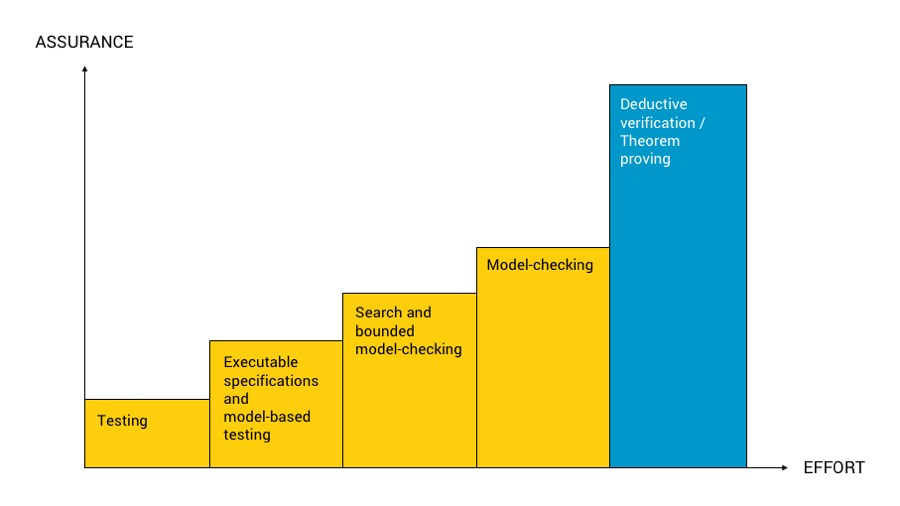
\includegraphics[width=\linewidth]{assets/verification.png}
%  \caption{Different verification methods and how they generally compare with respect to the confidence-effort trade off.}
%  \label{fig:verification}
%\end{figure}

The strongest guarantees, and thus the highest degree of trustworthiness, are obtained through deductive verification and theorem proving. In deductive verification, systems are modeled and specified inside expressive formal logical systems, and verified in a similar way to how mathematicians prove theorems - in principle by elaborating proofs of statements step-by-step. Among tools for deductive verification, \emph{proof assistants}~\cite{Geuvers2009,Harrison2014} offer the smallest trusted computing base necessary to trust verified statements, realized in modestly-sized trusted checkers that only assume a small set of axioms accepted by most mathematicians. Although they provide such strong guarantees, proof assistants can offer extensive automation and user support. Nevertheless, the process of figuring out what properties are relevant, how these properties are specified and building up their proofs normally requires a great deal of human ingenuity and experience. However, once everything is specified, proofs developed in proof assistants can be machine-checked, and persisted to serve as independently verifiable evidence that the properties hold for the given system~\cite{Pollack1998}.

\subsection{Coq and the Mathematical Components Library}

Coq can be viewed as consisting of, on the one hand, a small and powerful purely functional programming language, and on the other hand, a system for specifying and proving properties. A Coq user writes functions and data and then interactively constructs the proof of a theorem by trying different proof tactics that transform the state of the in-progress proof. Coq only accepts the theorem after its checker has been run on the purported proof. The Mathematical Components (MathComp) project~\cite{MathComp} provides a set of Coq libraries with standard mathematical data structures such as sequences, finite sets, and multisets, packaged to facilitate extension and formal proofs~\cite{Garillot2009}. Proofs in MathComp are written in the SSReflect proof language~\cite{Gonthier2010}, which extends Coq's proof tactic language.

%Coq has previously been used to develop a verified C compiler, formally prove mathematical results such as the four-color theorem, and verify distributed protocols (see, for example, our previous Casper formal verification effort for the Ethereum Foundation).

[Mathematical Components]

%We employ several existing Coq libraries which already formalized
%the majority of the mathematics we need to define and reason about Casper.
%Mathematical Components~\cite{MathComp} is a Coq library based on packaging
%mathematical structures and results in the form of Coq \emph{canonical
%  structures}, which can be reused and specialized when
%required~\cite{Garillot2009}.
%The library was used by Gonthier~et~al.\ to capture finite group theory and
%prove fundamental results in abstract algebra~\cite{Gonthier2013}.
%In addition to structures from abstract algebra, the library also contains
%encodings of and results about many standard data structures, such as numbers,
%lists, and finite sets.
